%\documentclass[10pt, a4paper]{article}
\documentclass[submit]{smj}

\usepackage[utf8]{inputenc}
\usepackage{amsmath, amssymb, amsthm, bbm}
\usepackage{xcolor}
\usepackage{graphicx}
\usepackage[authoryear]{natbib}
\usepackage{apalike}
\usepackage{relsize}
\usepackage{array}
\usepackage{multirow}
%\usepackage{showlabels}
\usepackage{setspace}
\usepackage[normalem]{ulem}
\usepackage{xspace}
%Add line numbering
%Line numbering can be incorporated by using the lineno package. Add these statements in the preamble:
%\usepackage{lineno}
%\linenumbers

%\usepackage[nomarkers,figuresonly]{endfloat}

\DeclareMathOperator*{\argmax}{arg\,max}

\newtheorem{prob}{Problem}
\newtheorem{prop}{Proposition}
\newtheorem{definition}{Definition}
\theoremstyle{definition}
\newtheorem{defn}{Definition}[section]
%%%%% bold symbol in math enviornment
\newcommand{\m}[1]{\boldsymbol{#1}}

\newcommand{\fmm}{\textsc{fmm}\xspace}
\newcommand{\X}{\text{\textbf{X}}}
\newcommand{\pkg}[1]{{\fontseries{b}\selectfont #1}} 

\Title{Merging the components of a finite mixture using  posterior probabilities}
\TitleRunning{Merging the components of \fmm}
\Author{Marc Comas-Cufí\Affil{1}, Josep A. Martín-Fernández\Affil{1}, Glòria Mateu-Figueras\Affil{1}}
\AuthorRunning{Marc Comas-Cufí \textrm{et al.}}

\Affiliations{
\item Department of Computer Sciences, Applied Mathematics and Statistics, 
      Polytechnic School, 
      University of Girona,
      Spain
}

\CorrAddress{Josep A. Martín-Fernández, Department of Computer Science, Applied Mathematics and Statistics,
      University of Girona, P-IV, Campus Montilivi, E-17071 Girona, Spain}
\CorrEmail{jamf@imae.udg.edu}
\CorrPhone{(+34)\;972\; 418\;426}
\CorrFax{(+34)\;972\;418\;792}

\Abstract{
Methods in parametric cluster analysis commonly assume that data can be modelled by means of a finite mixture of distributions. Different authors show that associating each mixture component to one cluster is frequently misleading because different mixture components overlap forming a unique cluster. A generic approach to build a hierarchy of mixture components generalises the most important techniques earlier proposed in the literature. Using the information provided by the posterior probabilities an iterative merging process constructs the clusters. The generic approach permits to define other merging indices. A new approach based in the log-ratio of posterior probabilities is introduced. Simulated and real datasets are used to illustrate the performance.
}

\Keywords{
Model-based clustering; Mixture model; Hierarchical clustering; Multilayer mixture; Merging components
}
\begin{document}

%\begin{spacing}{1.9}
%%%%%%% BEGIN SPACING


\pagenumbering{arabic}

\maketitle

\section{Introduction}


% Mixture models
A common approach in parametric cluster analysis assumes data can be modelled by means of a \emph{finite mixture of distributions} \citep{fraley2002model, punzo2014flexible}, also called \emph{finite mixture model} (\fmm). A \fmm is a probability distribution whose probability density function (pdf) is a linear combination of different distributions with same domain $\mathbb{X}$. More precisely, the pdf $f$ of a \fmm is
\begin{equation}\label{mixt}
f(\;\cdot\; ; \pi_1, \dots, \pi_k, \m\Theta) = \pi_1 f_1(\;\cdot\; ; \m\theta_1) + \dots + \pi_k f_k(\;\cdot\; ; \m\theta_k),
\end{equation}
where $\m\Theta =\{ \m\theta_1, \dots, \m\theta_k\}$, $\m\theta_j$ are the parameters of pdf $f_j$, $1\leq j \leq k$, and $\pi_j$ is the ``weight'' of component $f_j$. Restriction $\sum_{\ell = 1}^k \pi_\ell = 1$ guarantees that  $\int_{\mathbb{X}}f = 1$. Originally, the clustering algorithm based on a \fmm follows two steps:
\begin{enumerate}
\item using the information provided by a sample $\X=\{\m x_1, \dots, \m x_n\}$, to calculate estimates $\hat{\pi}_1, \dots, \hat{\pi}_k$ and $\hat{\m\Theta}$ of parameters $\pi_1, \dots, \pi_k$ and $\m\Theta$, and
\item to classify each observation $\m x_i \in \X$ according to the criterium of maximizing the posterior probability
\[
\tau_{ij}= \frac{ \hat{\pi}_j f_j(\m x_i ; \hat{\m\theta}_j) }{\sum_{\ell=1}^k \hat{\pi}_\ell f_\ell(\m x_i ; \hat{\m\theta}_\ell) },
\]
that is, one observation $\m x_i$ is classified to cluster $c$ if
\begin{equation}\label{map_criteria}
c = \argmax_{j=1}^k \tau_{ij}.
\end{equation}
\end{enumerate}
Note that in this process, the number of clusters $k$ is equal to the number of mixture components. \cite{mclachlan2014components} presents a recent review of different approaches used to decide the value of $k$. From the reviewed approaches, we use the Bayesian Information Criterion (BIC) to fit the number of mixture components.\footnote{Tenim la següent frase a Baudry, 2010 justificant la selecció del BIC: \emph{Keribin (1998, 2000) has shown that under certain regularity conditions
the BIC consistently estimates the number of mixture components, and numerical experiments
show that the BIC works well at a practical level (Fraley and Raftery 1998; Biernacki et al.
2000; Steele 2002).}}

On the other hand, \cite{lee2004combining,hennig2010methods,baudry2010combining,melnykov2013distribution,pastore2013merging} propose to separate the concepts of cluster and mixture component. The authors show that associating each mixture component to one cluster can be misleading because frequently different mixture components are so overlapped that they can be considered as a unique cluster. In other words, one cluster could be formed by the result of merging two different mixture components. According to this approach, the \fmm clustering algorithm is completed with a third step:

\begin{itemize}
\item[3.] to analyse which of the $k$ mixture components should be merged to form $k'$ clusters, $k' \leq k$.
\end{itemize}

The crucial point of this new step is how to decide which components have to be merged. In this article we introduce a generic approach that generalises methods given by \cite{baudry2010combining}, \cite{hennig2010methods} and \cite{longford2014}. With this approach, the analyst can define its own criteria, for example, a criteria based in log-ratio transformations of posterior probabilities \citep{aitchison1986statistical}. Using this new generic approach for merging components one can build a hierarchy over the set of mixture components. From this hierarchical structure, the analyst can decide the final classification.

The paper is organised as follows: in Section~\ref{definitions} some definitions and notations used throughout this paper are introduced. In Section~\ref{generic_merging} the generic merging approach is presented. It is shown how most important criteria from literature reduce to this generic approach. Using the generic merging approach, Section~\ref{logratio_section} presents a new family of criteria based on the log-ratio approach. In Section~\ref{merging_examples_dist}, we present two examples to illustrate the algorithm with different types of mixture distributions. To conclude, final remarks are given in Section~\ref{remarks}.

\section{Definitions and notation}\label{definitions}

%
Let $\mathcal{I}^k = \{1, \dots, k\}$. A \emph{partition} of $\mathcal{I}^k$ of size $s$, $\mathcal{P}_s$, is the disjoint union of subsets $I_p$, called \emph{parts}. More formally, $\mathcal{P}_s$ is a set with $s$ subsets $I_p$  that $\bigcup_{I_p \in \mathcal{P}_s} I_p = \mathcal{I}^k$ and for any two parts $I_a, I_b \in \mathcal{P}_s$ with $a \neq b$, $I_a \cap I_b = \emptyset$ holds. Given a partition  $\mathcal{P}_s$, the pdf $f$ of a \fmm (Equation~\ref{mixt}) can be rewritten as
\begin{equation}
f = \pi_{I_1} f_{I_1}(\;\cdot\;; \m\Theta) + \dots + \pi_{I_s} f_{I_s}(\;\cdot\;; \m\Theta),
\label{mixt_part}
\end{equation}
where $f_{I_p}(\;\cdot\;;  \m\Theta) = \sum_{j \in I_p} \frac{\pi_j}{\pi_{I_p}} f_j(\;\cdot\; ; \m\theta_j)$ and $\pi_{I_p} = \sum_{\ell \in I_p} \pi_\ell$. Note that using this notation each $f_{I_p}(\;\cdot\;;  \m\Theta)$ is also a \fmm. Because each part $I_p$ defines a single component $f_{I_p}$, if there is no confusion, we use $I_p$ referring either to the part $I_p$ or to the component $f_{I_p}$.



A \emph{hierarchical sequence of partitions of $\mathcal{I}^k$}, is a sequence $\mathcal{P}_1, \dots, \mathcal{P}_k$ verifying that
\begin{itemize}
\item $\mathcal{P}_1$ is the one-part partition $\mathcal{P}_1 = \{ \mathcal{I}^k \}$,
\item if a part $I_p \in \mathcal{P}_{s-1}$ then either there is a part $I_a \in \mathcal{P}_{s}$ with $I_p = I_a$ or there are two parts $I_a, I_b \in \mathcal{P}_s$ with $I_p = I_a \cup I_b$, and
\item $\mathcal{P}_k= \{ \{1\},\{2\}, \dots, \{k\} \}$.
\end{itemize}



One can extend Equation~\ref{map_criteria} in terms of partitions. Indeed, let $\X = \{\m x_1,\dots, \m x_n\}$ be a sample formed by observations of $\mathbb{X}$. Given a partition $\mathcal{P}_s = \{ I_1, \dots, I_s \}$, we define the posterior probability of $\m x_i$ being classified to part $I_p\in \mathcal{P}_{s}$ as
\[
\tau_{i I_p} =  \frac{ \hat{\pi}_{I_p} f_{I_p}(\m x_i; \hat{\m\Theta}) }{\sum_{\ell=1}^s \hat{\pi}_{I_\ell} f_{I_\ell}(\m x_i; \hat{\m\Theta})}
\]
where $\hat{\pi}_{I_p} = \sum_{\ell \in I_p} \hat{\pi}_\ell$.\footnote{No sé si caldria comentar-ho. A Hennig, 2010 es diu que no hi ha manera des d'un punt de vista freqüentista de decidir quina partició és millor. \emph{From a purely frequentist perspective, modelling f as the underlying data generating distribution and the $(\pi_i, \m \mu_i, \m\Sigma_i)$, $i = 1,\dots,s$, as fixed parameters, there is no statistical way to distinguish “true” cluster mixtures $f^*_1 ,\dots, f^*_k$ (aquí $f_{I_1} ,\dots, f_{I_k}$) from any others. It rather has to be decided by the statistician under which conditions different Gaussian mixture components should be regarded as a common cluster. This cannot be estimated from the data, but needs to take into account the (usually subject-matter dependent) cluster concept of interest. It is well known that there is no objective unique definition of what a “true cluster” is, so there is necessarily a subjective component in this decision.}}

For the partition  $\mathcal{P}_s$, we define the posterior probability vector associated to observation $\m x_i$ as
\begin{equation}\label{ppv}
\m\tau_{i \mathcal{P}_s} = \left(\tau_{i I_1} , \dots, \tau_{i I_s}  \right).
\end{equation}
The posterior probability vector $\m \tau_{i \mathcal{P}_s}$ denotes the conditional probability that $\m x_i$ arises from mixture components $f_{I_1}, \dots, f_{I_s}$. Since $\mathcal{P}_s$ is a partition $\sum_{p=1}^s \tau_{i I_p} = 1$ holds  for $1 \leq i \leq n$. Similarly to Equation~\ref{map_criteria}, the posterior probability vectors $\m\tau_{i \mathcal{P}_s}$ can be used to classify, $\m x_i \in \X$ will be classified to the cluster $c$ if
\begin{equation}\label{cluster_criteria}
c= \argmax_{p=1}^s \{ \tau_{i I_p} \}.
\end{equation}

Let $\text{\textbf{T}}_{\mathcal{P}_s}$ be the matrix with $n$ rows and $s$ columns formed by the vectors of posterior probabilities $\m \tau_{i\mathcal{P}_s}$ associated to partition $\mathcal{P}_s$. For example, $\text{\textbf{T}}_{\mathcal{P}_k}$ is the initial matrix, when the number of components and clusters are equal. Importantly, by Equation \ref{ppv}, any matrix $\text{\textbf{T}}_{\mathcal{P}_s}$ can be obtained from matrix $\text{\textbf{T}}_{\mathcal{P}_k}$ respectively aggregating the corresponding columns of part $I_1, \dots, I_s$.


\section{Generic approach}\label{generic_merging}
\subsection{Discusió sobre el criteria de merging}

In this section we define a function measuring how reasonable is that two different components, $f_{I_a}$ and $f_{I_b}$, define a single cluster. In the literature, different methodologies have been described to decide if two components define a single cluster. Most of this methodologies are described in Hennig, 2010. The author separate them between two categories: models based on modality and models based on missclassification probabilities.


Es vol una funció per mesurar quan bo és considerar dos components com a un mateix cluster.

\subsection{General merging criteria}\label{merging_criteria}

Let $\text{\textbf{X}} = \{\m x_1,\dots,\m x_n \}$ be a sample defined in  a domain $\mathbb{X}$ and let $f$ be a \fmm with $k$ components defined on $\mathbb{X}$ (Equation~\ref{mixt}). Given a partition $\mathcal{P}_s = \{I_1, \dots, I_s\}$, let $\m\tau_{i \mathcal{P}_s}= \left( \tau_{i I_1} , \dots, \tau_{i I_s}  \right)$ be the posterior probability vector associated to observation $\m x_i$ for $i$, $1\leq i \leq n $.

For a partition $\mathcal{P}_s$  and matrix of posterior probabilities $\text{\textbf{T}}_{\mathcal{P}_s}$ we propose to merge those two parts $I_a, I_b \in \mathcal{P}_s$ maximising the weighed mean
\begin{equation}\label{unifying_equation}
S_{\omega, \lambda}( \text{\textbf{T}}_{\mathcal{P}_s},  I_a,  I_b) = \frac{\sum_{i=1}^n \omega(\m\tau_{i \mathcal{P}_s}, I_a, I_b) \; \lambda(\m\tau_{i \mathcal{P}_s}, I_a, I_b)}{\sum_{i=1}^n \omega(\m\tau_{i \mathcal{P}_s}, I_a, I_b) }.
\end{equation}
where $\omega(\m\tau_{i \mathcal{P}_s}, I_a, I_b)$ is a non-negative function and $\lambda(\m\tau_{i \mathcal{P}_s}, I_a, I_b)$ is a function measuring the preferences for the researcher in merging component $I_a$ and $I_b$.


Starting from partition $\mathcal{P}_k = \{ \{1\}, \dots, \{k\} \}$, where the number of clusters is equal to the number of components, we merge two parts according to the maximum of Equation~\ref{unifying_equation}. Iteratively repeating this process until partition $\mathcal{P}_1$ is obtained, the algorithm builds an agglomerative hierarchical sequence of partitions. Remarkably, by the definition of functions $\omega$ and $\lambda$, the process only depends on the posterior probability vectors $\text{\textbf{T}}_{\mathcal{P}_s}$. Indeed, the behaviour of function $S$ is completely determined by the choice of function $\omega$ and $\lambda$.


Function $\omega(\m\tau_{i \mathcal{P}_s},  I_a,  I_b)$ is a weigh function. It permits to modify the influence each posterior probability vector $\m\tau_{i \mathcal{P}_s}$ has to calculate Equation~\ref{unifying_equation} for parts $I_a$ and $I_b$, we call the value of Equation~\ref{unifying_equation} \emph{the $S$-value from $I_a$ to $I_b$}. Function $\lambda(\m\tau_{i \mathcal{P}_s},  I_a,  I_b)$ is an utility function. It measures our preferences to consider components $f_{I_a}$ and $f_{I_b}$ as a single component, and therefore, to model a single cluster by means of a single component $f_{I_a \cup I_b}$.



\subsection{Minimising the final entropy}
\label{entropy_section}

\cite{baudry2010combining} propose an algorithm to build a hierarchical sequence of partitions based on the concept of entropy. The Shannon entropy of a posterior probability vector $\m\tau_{i \mathcal{I}_s} = \left( \tau_{i I_1} , \dots, \tau_{i I_s}  \right)$ is
\[
\text{Ent}( \m\tau_{i \mathcal{P}_s} ) = -\sum_{j=1}^s \tau_{i I_j}  \log(\tau_{i I_j} ).
\]

The entropy can be interpreted as a measure of similarity between a probability vector and the probability vector $\m\tau^0_{s}=\left(\frac{1}{s}, \dots, \frac{1}{s}\right)$, taking the maximum value when $\text{Ent}\left( \m\tau^0_{s} \right) = -log(s)$. Starting from partition $\mathcal{P}_k = \{ I_1, \dots, I_k\}$ the algorithm iteratively merges  the two mixture components optimising the overall entropy. Let $\mathcal{P}_{s-1}^{I_a\cup I_b}$ be the partition obtained after merging components $I_a$ and $I_b$ from $\mathcal{P}_s$. The parts $I_a$ and $I_b$ merged minimises the expression
\[
\sum_{i=1}^n \text{Ent}( \m\tau_{i \mathcal{P}_{s-1}^{I_a\cup I_b}} ).
\]

According to \cite{baudry2010combining}, minimizing previous expression is equivalent to maximise the loss of entropy, that is, to maximise the difference
\[
\sum_{i=1}^n  \left\{ \text{Ent}( \m\tau_{i \mathcal{P}_s} ) - \text{Ent}( \m\tau_{i \mathcal{P}_{s-1}^{I_a\cup I_b}} ) \right\}.
\]
which can be written only in terms of $\tau_{i I_a}$  and $\tau_{i I_b}$ as
\begin{equation}\label{entropy}
\sum_{i=1}^n   \left\{(\tau_{iI_a}+\tau_{iI_b}) \log(\tau_{iI_a} + \tau_{iI_b}) - \left[\tau_{iI_a} \log(\tau_{iI_a}) + \tau_{iI_b} \log(\tau_{iI_b})\right] \right\}.
\end{equation}
We define function $\lambda$ as
\[
\lambda(\m\tau_{i \mathcal{P}_s},  I_a,  I_b) =  (\tau_{iI_a}+\tau_{iI_b}) \log(\tau_{iI_a} + \tau_{iI_b}) - \left[ \tau_{iI_a} \log(\tau_{iI_a}) + \tau_{iI_b} \log(\tau_{iI_b}) \right],
\]
and function $\omega$ constant, for example 
\[
\omega(\m\tau_{i \mathcal{P}_s},  I_a,  I_b) = 1.
\]

In this case Equation~\ref{unifying_equation} takes the form
\[
\begin{split}
S_{\omega, \lambda}( \m\tau_{\mathcal{P}_s},  I_a,  I_b) = \frac{1}{n} \sum_{i=1}^n & \left\{(\tau_{iI_a}+\tau_{iI_b}) \log(\tau_{iI_a} + \tau_{iI_b}) - \right.\\ 
&\quad \left.\left[ \tau_{iI_a} \log(\tau_{iI_a}) + \tau_{iI_b} \log(\tau_{iI_b}) \right]\right\}.
\end{split}
\]


\subsection{Maximising the misclassification probability}
\label{missclassification_section}

A different approach is introduced by \cite{hennig2010methods}. He proposes to merge the components $I_a$ and $I_b$ from $ \mathcal{P}_s$ that maximise \emph{the probability of classifying to component $I_b$ an observation generated from component $\hat{f}_{I_a}$ }.

To estimate this probability,  \cite{hennig2010methods} uses a consistent estimator, the Directed Estimated Misclassification Probabilities (DEMP). The estimator is
\[
\frac{ \frac{1}{n} \sum_{i=1}^n {\tau_{iI_a} \mathbbm{1}\left( \forall j\; \tau_{i I_{b}} \geq \tau_{iI_j} \right)}}{ \hat{\pi}_{I_a}},
\]
where $\mathbbm{1}\left( \cdot \right)$ is the indicator function. Because $ \hat{\pi}_{I_a} = \frac{1}{n} \sum_{i=1}^n \tau_{iI_a}$, the previous estimator can be written in terms of the posterior probability vector as
\begin{equation}\label{demp_criteria}
\frac{ \sum_{i=1}^n {\tau_{iI_a} \mathbbm{1}\left( \forall j\; \tau_{i I_{b}} \geq \tau_{iI_j} \right)}}{\sum_{i=1}^n \tau_{iI_a} }.
\end{equation}

In consequence, the DEMP estimator is included in the generic criteria when
\begin{equation}\label{lambda_demp}
\lambda(\m\tau_{i \mathcal{P}_s},  I_a,  I_b) = \mathbbm{1}\left( \forall j\; \tau_{i I_{b}} \geq \tau_{iI_j} \right)
\end{equation}
and
\[
\omega(\m\tau_{i \mathcal{P}_s},  I_a,  I_b) =  \tau_{iI_a}.
\]

A variation of \cite{hennig2010methods} approach is proposed by \cite{longford2014}. Instead of considering function $\lambda$ given by Equation~\ref{lambda_demp} they propose to measure the confusion between $I_a$ and $I_b$ with function $\lambda$ given by
\[
\lambda(\m\tau_{i \mathcal{P}_s},  I_a,  I_b) = \frac{\tau_{iI_b}}{\tau_{iI_a} + \tau_{iI_b}},
\]
giving another example of function $S_{\omega, \lambda}( \m\tau_{\mathcal{P}_s},  I_a,  I_b)$.

Finally, without restricting  the posterior probability of begin classified to component $I_b$, a simple modification to the approach proposed by \cite{longford2014} can be introduced by defining
\[
\lambda(\m\tau_{i \mathcal{P}_s},  I_a,  I_b) = \tau_{iI_b}.
\]
If combined with $\omega(\m\tau_{i \mathcal{P}_s},  I_a,  I_b) =  \tau_{iI_a}$ end ups with a very simple approach to build a hierarchy.

\subsection{$\omega$ function alternative}


An important difference between the approach presented in Section~\ref{entropy_section} \citep{baudry2010combining} compared to the one presented in Section~\ref{missclassification_section} \citep{hennig2010methods} is that the former one is symetric, that is
\[
S_{\omega, \lambda}( \m\tau_{\mathcal{P}_s},  I_a,  I_b) = S_{\omega, \lambda}( \m\tau_{\mathcal{P}_s},  I_b,  I_a).
\]
In contrast, DEMP approach has different values depending on the merging order.

Function $\omega$ plays an important role for the symetry of the method. In general, if $\omega$ is constant and $\lambda$ is symetric the resulting function $S_{\omega, \lambda}( \m\tau_{\mathcal{P}_s},  I_a,  I_b)$ is symetric.

Motivation behind function $\omega(\m\tau_{i \mathcal{P}_s},  I_a,  I_b) = \tau_{iI_a}$ in \cite{hennig2010methods} is to give more weight to those observations more related to partition $I_a$. A more extremal asymetric weighting can be introduced considering only those observation having maximum $ \tau_{iI_a}$, that is
\[
\omega(\m\tau_{i \mathcal{P}_s},  I_a,  I_b) = \mathbbm{1}\left( \forall j\; \tau_{i I_{a}} \geq \tau_{iI_j} \right).
\]
This approach emphasize those observations that in the current stage are classified to component $I_a$.


\section{The logratio approach}\label{logratio_section}

The generic expression of $S_{\omega, \lambda}( \m\tau_{\mathcal{P}_s},  I_a,  I_b)$ (Equation~\ref{unifying_equation}) permits to extend the criteria for merging components to expressions defined by the analyst. \cite{aitchison1986statistical} introduces a serie of tools to study samples defined in the Simplex space $\mathcal{S}^d$, i.e $\mathcal{S}^d = \{ (x_1,\dots, x_d) \;|\; x_i > 0 \text{ and } \sum_{i=1}^k x_i = 1 \}$. 

In this section we are interested in different approaches to measure the chances of merging two parts $I_a$ and $I_b$ taking into an account that the posterior probability vector are observations in the Simplex space. In other words we are interested in defining functions $\lambda$ which takes into an account the geometric structure of $\mathcal{S}^d$. We are going to define two new measures, the first ones is motivated by the Entropy notion introduced in \ref{entropy_section}, the second is based on the misclassification definition given in Section~\ref{missclassification_section}.


In \cite{baudry2010combining} confusion between components is measured using the notion that the closer the posterior probability vector is from $(\frac{1}{s}, \dots, \frac{1}{s})$ the more confused are the components (higher is the Entropy). To measure the chances of confusing $I_b$ with $I_a$ we can measure how different is $(\frac{\tau_{i I_a}}{\tau_{i I_a} +\tau_{i I_b}}, \frac{\tau_{i I_b}}{\tau_{i I_a} + \tau_{i I_b}})$ from $(\frac{1}{2}, \frac{1}{2})$. That is, to restrict only on the probabilities associated to the components to be merged. To measure this difference we use the squared norm defined in the Simplex space. The squared norm of a posterior probability vector, $\| (\tau_{iI_a}, \tau_{iI_b}) \|^2$  defined by \cite{aitchison2002simplicial} is 
\[
\left\| (\tau_{iI_a}, \tau_{iI_b}) \right\|^2 = \log^2 \left(\frac{ \tau_{iI_b} }{ \tau_{iI_a} }\right).
\]

Because we are interested on merging those components $I_a$ and $I_b$ with lower norm and Equation~\ref{unifying_equation} is maximized, we propose
\[
\lambda(\m\tau_{i \mathcal{P}_s},  I_a,  I_b) = -\left\| (\tau_{iI_a}, \tau_{iI_b}) \right\|^2 = -\log^2 \left(\frac{ \tau_{iI_b} }{ \tau_{iI_a} }\right)
\]


The second log-ratio approach is inspired in the notion of confusion \citep{hennig2010methods} between two components $I_a$ and $I_b$. Conditioning that the observation is generated by $I_a$ we propose to measure how likely is to classify an observation to $I_b$ by measuring the relative difference between $\tau_{i I_b}$ and $\tau_{i I_a}$, that is 
\[
\lambda(\m\tau_{i \mathcal{P}_s},  I_a,  I_b) = \log \left(\frac{ \tau_{iI_b} }{ \tau_{iI_a} }\right).
\]


Due the two different methods use logratios they take into an account the geometric properties of the Simplex space \citep{aitchison2002simplicial}.  Working with logratios between components we guarantee \emph{subcompositional coherence}  \citep{aitchison1986statistical}. Formally, in this scenario subcompositional coherence can be defined as:

\begin{defn}
Let $\mathcal{H}$ be a hierarchical sequence of partitions obtained from posterior probability vectors $\left\{ \left(\tau_{i1}, \dots, \tau_{ik} \right)\right\}_{1\leq i \leq n}$ using a merging approach $M$. Let $I = \{j_1, \dots, j_s\}$ be one part in one partition of $\mathcal{H}$. A method is \emph{subcompositional coherent} if the hierarchy sequence of partitions obtained  from posterior probability vectors $\left\{ \left(\tau_{ij_1}, \dots, \tau_{ij_s} \right)\right\}_{1\leq i \leq n}$ is contained in $\mathcal{H}$.
\end{defn}

Another interesting feature when logratio approach is used is the \emph{scale invariance} property, formally
\[
S_{\omega, \lambda}( \m\tau_{\mathcal{P}_s},  I_a,  I_b) = S_{\omega, \lambda}(k\cdot \m\tau_{\mathcal{P}_s},  I_a,  I_b) \text{ for $k>0$.}
\] 

Meaning that the approach is not restricted to posterior probability vectors but to any other kind of vector giving relative information between each mixture component. Therefore, the methods considered here are suitable to be applied in more general scenarios such that those were instead of posterior probability vectors different weights are given to each part (e.g. weights in fuzzy clustering).

The selection of $\omega(\m\tau_{i \mathcal{P}_s},  I_a,  I_b)$ is of special importance in the logratio approach. When we are considering to merge two components $I_a$ and $I_b$, the ratio for observations that are not representative of this two components (observations far from been classidied into $I_a$ or $I_b$) should be unweight. The main reason is that this posterior probabilitites are subject to a high amount of variability due the small posterior probabilities $\tau_{iI_a}$ and $\tau_{iI_b}$ involved.

Noting also that when $\omega(\m\tau_{i \mathcal{P}_s},  I_a,  I_b) =  \tau_{iI_a}$ and $\lambda(\m\tau_{i \mathcal{P}_s},  I_a,  I_b) = \log \left(\frac{ \tau_{iI_b} }{ \tau_{iI_a} }\right)$ are considered, Equation~\ref{unifying_equation} results in
\[
S_{\omega, \lambda}( \m\tau_{\mathcal{P}_s},  I_a,  I_b) = \frac{\sum_{i=1}^n\tau_{iI_a}  \log \left(\frac{ \tau_{iI_b} }{ \tau_{iI_a} }\right)}{\sum_{i=1}^n \tau_{iI_a}}.
\]
For a fixed component $I_a$, the expression in the numerator has the flavour of the Kullback-Leibler divergence (in negative sign) comparing the distribution of classifiying observations $x_i \in X$ to $I_a$ against the distributions of classifying the same observations to $I_b$.

\section{Merging components in a finite mixture: examples}\label{merging_examples_dist}

\subsection{Merging components in a mixture of Gaussian distributions}

Following \cite{baudry2010combining} consider the bivariate Gaussian mixture of six components
\[
f= \sum_{j=1}^6 \pi_j \phi(\;\cdot\; ;  \m\mu_j, \m\Sigma_j)
\]
with parameters shown at Table~\ref{pars_table}. 

\begin{table}[t]
\centering
\begin{tabular}{rrrrrrr}
  \hline
$j$ & $\pi_j$ & $\mu_{j x_1}$ & $\mu_{j x_2}$ & $\sigma^2_{j x_1}$ & $\sigma^2_{j x_2}$ & $\rho_{j x_1 x_2}$ \\ 
  \hline
  1 &  $1/6$ &     0 &     0 &    50 &     5 &     0 \\ 
  2 &  $1/6$  &     0 &    40 &     5 &    50 &     0 \\ 
  3 &  $1/6$  &    40 &    40 &     5 &    50 &     0 \\ 
  4 &  $1/6$  &     0 &     0 &     5 &    50 &     0 \\ 
  5 &  $1/6$  &    40 &     0 &    50 &     5 &     0 \\ 
  6 &  $1/6$  &    40 &    40 &    50 &     5 &     0 \\ 
   \hline
\end{tabular}
\caption{Parameters defining a two dimensional Gaussian mixture with six components. The parameters $\m\mu_j$ and $\m\Sigma_j$ are expressed in terms of the univariate means $\mu_{j x_1}$, $\mu_{j x_2}$, the univariate variances $\sigma^2_{j x_1}$, $\sigma^2_{j x_2}$ and the correlation between $x_1$ and $x_2$, $\rho_{j x_1 x_2}$.}
\label{pars_table}
\end{table}


Let the parameters of $f$ be known. Figure~\ref{ex_mixture} shows a random sample \textbf{X} together with the iso-density curves of the estimated \fmm. We are interested in clustering sample \textbf{X}.

\begin{figure}[htbp]
\begin{center}
\begin{tabular}{cc}
 %   6 toy mixture
  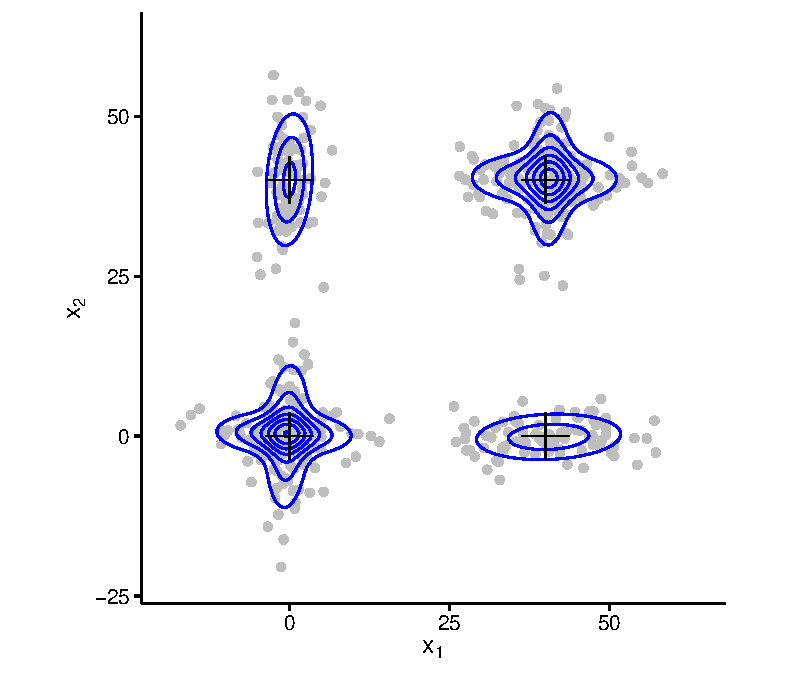
\includegraphics[width=0.7\textwidth]{figures/partition-example-mixture.pdf} \\
 \end{tabular}
 \caption{Density of Gaussian mixture of 6 components. Sample mean estimated of each component is represented by '+'.}\label{ex_mixture}
\end{center}
\end{figure}

The initial partition  $\mathcal{P}_6 = \{ \{1\},\{2\}, \{3\}, \{4\}, \{5\}, \{6\} \}$  by Equation~\ref{cluster_criteria} yields to a six clusters were each component is associated to one cluster as shown in Figure~\ref{ex_one_one}.

\begin{figure}[h]
\begin{center}
\begin{tabular}{cc}
 %   6 toy mixture
  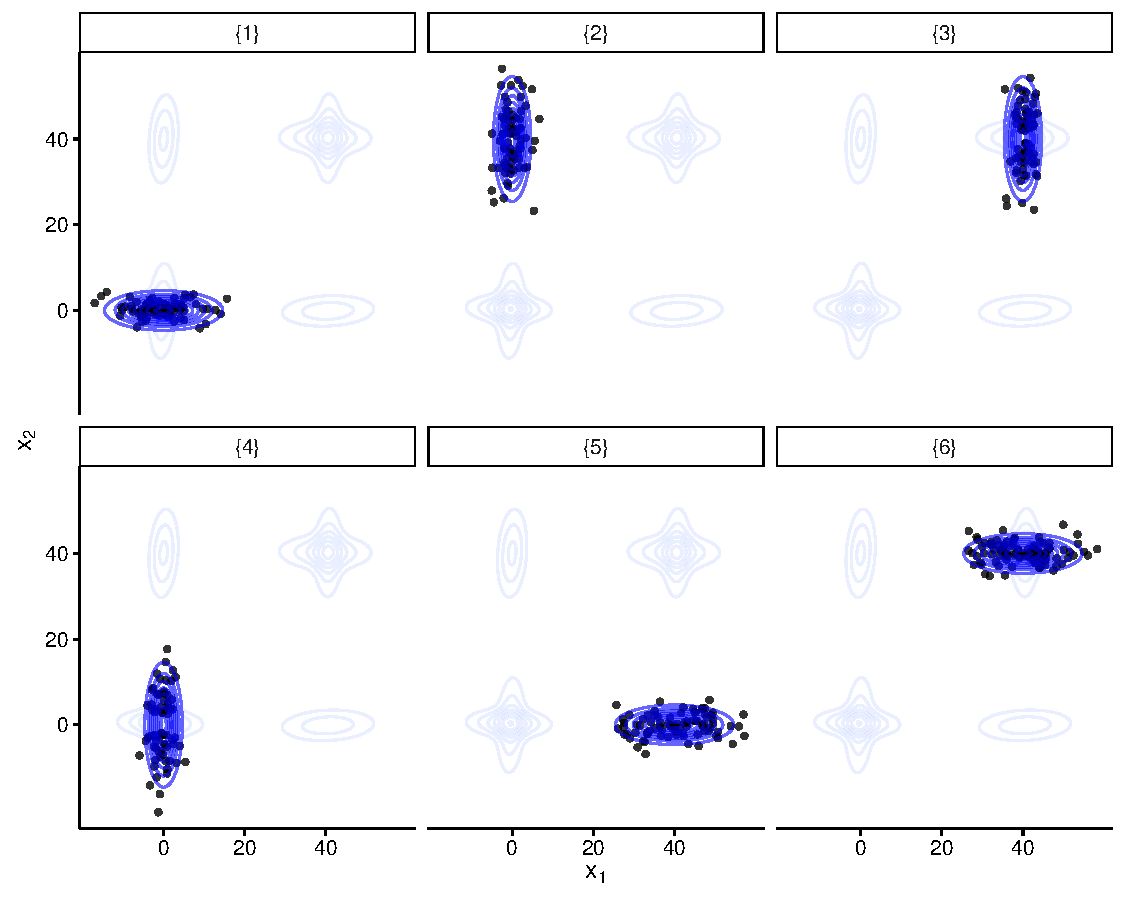
\includegraphics[width=\textwidth]{figures/partition-example-part6.pdf} \\
 \end{tabular}
 \caption{One cluster corresponds to one component}\label{ex_one_one}
\end{center}
\end{figure}

\cite{baudry2010combining} proposed the Entropy approach, in Section~\ref{entropy_section} we have seen the approach is equivalent to consider \[\omega = 1\] and \[\lambda = (\tau_{iI_a}+\tau_{iI_b}) \log(\tau_{iI_a} + \tau_{iI_b}) - \left\{ \tau_{iI_a} \log(\tau_{iI_a}) + \tau_{iI_b} \log(\tau_{iI_b}) \right\}.\] Following this approach we obtained the sequential hierarchical partition given by 

\begin{equation}
\begin{array}{r c l}
\mathcal{P}_1 &=& \{\{1, 2, 3, 4, 5, 6\}\}, \\
\mathcal{P}_2 &=& \{\{1, 4, 2, 5\}, \{6, 3\} \},  \\
\mathcal{P}_3 &=& \{\{1, 4, 2\}, \{5\}, \{6, 3\} \}, \\
\mathcal{P}_4 &=& \{\{1, 4\},\{2\}, \{5\}, \{6, 3\} \}, \\
\mathcal{P}_5 &=& \{\{1\},\{2\},\{4\},\{5\},\{6,3\} \},\\
\mathcal{P}_6 &=& \{\{1\},\{2\},\{3\},\{4\},\{5\},\{6\}\}.
\end{array}
\label{hier_ex}
\end{equation}

In the partition $\mathcal{P}_4 = \{ \{1, 4\},\{2\}, \{5\}, \{3, 6\} \}$, the components 1 and 4 define a single cluster, as well as components 3 and 6. Using Equation~\ref{cluster_criteria} each observation $\m x_i$ is classified to one component. Figure~\ref{ex_two_one} shows the clustering with the iso-density curves defined by each component. In this case, clusters labeled $\{1,4\}$ and $\{3, 6\}$ are modelled by a mixture of two components. With partition $\mathcal{P}_4$ the clusters are modelled by $\fmm$s
\begin{itemize}
\item $f_{\{1,4\}} = \frac{1}{2} \phi(\;\cdot\; ;  \m\mu_1, \m\Sigma_1) + \frac{1}{2} \phi(\;\cdot\; ;  \m\mu_4, \m\Sigma_4)$, 
\item $f_{\{2\}} = \phi(\;\cdot\; ;  \m\mu_2, \m\Sigma_2)$, 
\item $f_{\{5\}} = \phi(\;\cdot\; ;  \m\mu_5, \m\Sigma_5)$ and
\item $f_{\{6,3\}} = \frac{1}{2} \phi(\;\cdot\; ;  \m\mu_6, \m\Sigma_6) + \frac{1}{2} \phi(\;\cdot\; ;  \m\mu_3, \m\Sigma_3)$.
\end{itemize}

\begin{figure}[h]
\begin{center}
\begin{tabular}{cc}
 %   6 toy mixture
  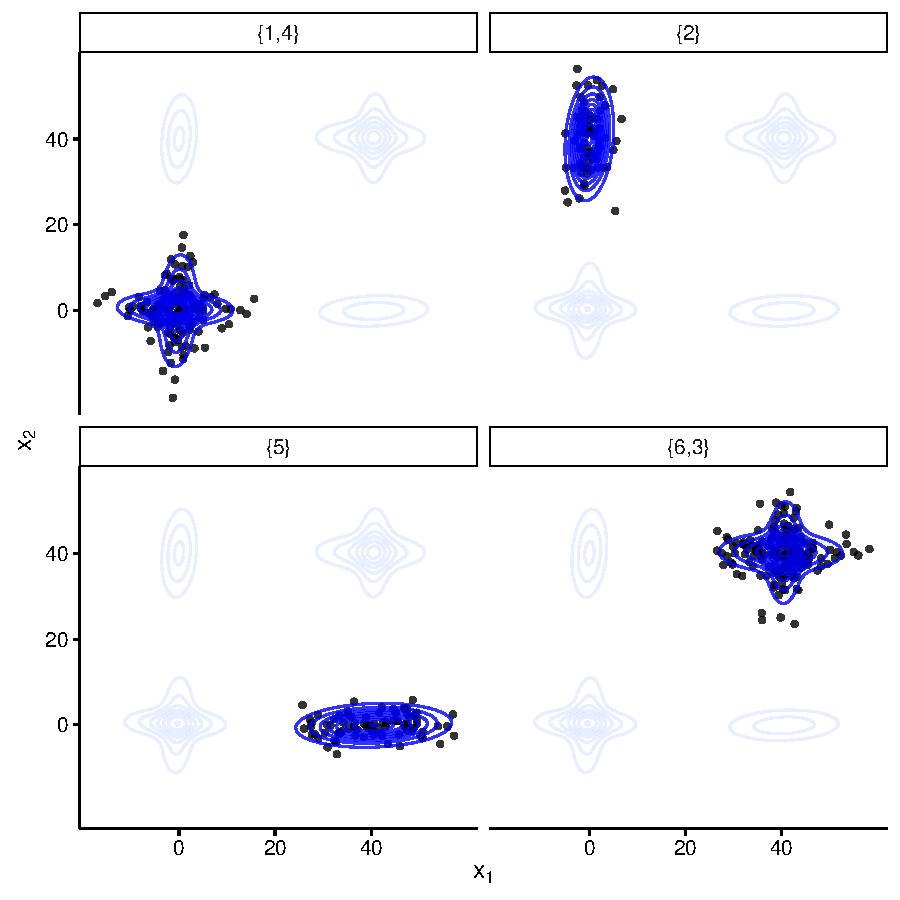
\includegraphics[width=0.65\textwidth]{figures/partition-example-part4.pdf} \\
 \end{tabular}
 \caption{One cluster corresponds to one or more components}\label{ex_two_one}
\end{center}
\end{figure}

If instead of using approach from Section~\ref{entropy_section} \citep{baudry2010combining} we consider DEMP approach from Section~\ref{missclassification_section} \citep{hennig2010methods}, we are setting \[\omega = \tau_{i I_a}\] and \[\lambda = \mathbbm{1}\left( \forall j\; \tau_{i I_{b}} \geq \tau_{iI_j} \right).\] In this case, the sequential hierarchical obtained is
\begin{equation}
\begin{array}{r c l}
\mathcal{P}_1 &=& \{\{1, 2, 3, 4, 5, 6\}\}, \\
\mathcal{P}_2 &=& \{\{1, 4, 2, 5\}, \{6, 3\} \},  \\
\mathcal{P}_3 &=& \{\{1, 4, 2\}, \{5\}, \{6, 3\} \}, \\
\mathcal{P}_4 &=& \{\{1, 4\},\{2\}, \{5\}, \{6, 3\} \}, \\
\mathcal{P}_5 &=& \{\{1, 4\},\{2\}, \{3\},\{5\},\{6\} \},\\
\mathcal{P}_6 &=& \{\{1\},\{2\},\{3\},\{4\},\{5\},\{6\}\}.
\end{array}
\end{equation}
This sequence only differs from the Baudry's in the partition $\mathcal{P}_5$.  

To detect the final number of clusters \cite{baudry2010combining} proposed to monitorize the values of function $S$ given by Equation~\ref{unifying_equation}. We refer to them as the $S$-values. Figure~\ref{gaussian_Svalues} shows the $S$-values using the Entropy and DEMP apporach. The largest change is detected in the step from 4 clusters to consider 3 clusters. Following \cite{baudry2010combining}, this reduction suggests that the correct number of clusters is given by 4 clusters.

\begin{figure}[t]
\begin{center}
\begin{tabular}{cc}
  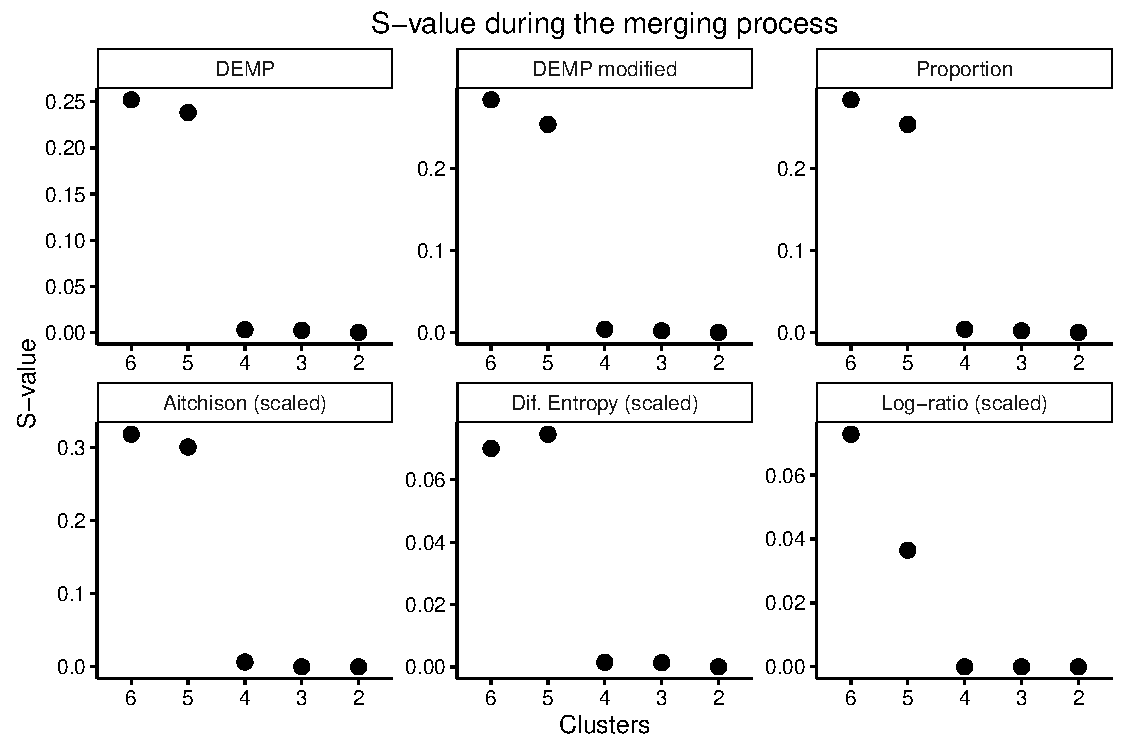
\includegraphics[width=0.85\textwidth]{figures/gaussian_Svalues.pdf} \\
 \end{tabular}
 \caption{S-values obtained using the approaches presented by Baudry et al. and Hennig labeled Entropy and DEMP respectively.}\label{gaussian_Svalues}
\end{center}
\end{figure}

\subsection{Merging components in a mixture of multinomial distributions}\label{multinom_example}

Merging approaches presented in this article rely on the vector of posterior probabilities this can be calculated for any finite mixture model. Therefore, the merging generic approach introduced in Section~\ref{generic_merging} can be used for any family of \fmm, for example a finite mixture of multinomial distribution.

Pigs dataset can be obtained from package \pkg{zCompositions} R package \citep{palarea2012zcompositions}. The dataset contains data of 29 sows. In different moments the pigs were recorded during 5 minutes and its current activity was registered. For each pig six locations were considered: straw bed (BED), half in the straw bed (HALF.BED), dunging passage (PASSAGE), half in the dunging passage (HALF.PASS), feeder (FEEDER) and half in the feeder (HALF.FEED).

We have used \pkg{mixtools} \citep{benaglia2009mixtools} to fit a mulitinomial mixture. 6 components were identified as optimum according to BIC criterion. In Figure~\ref{multinomial_mixture} the bar plot for each component is shown. That is considering Equation~\ref{map_criteria} or Equation~\ref{cluster_criteria} with partition $\mathcal{P}_6 = \{\{1\}, \{2\}, \{3\}, \{4\}, \{5\}, \{6\}\}$.

\begin{figure}[t]
\begin{center}
\begin{tabular}{cc}
  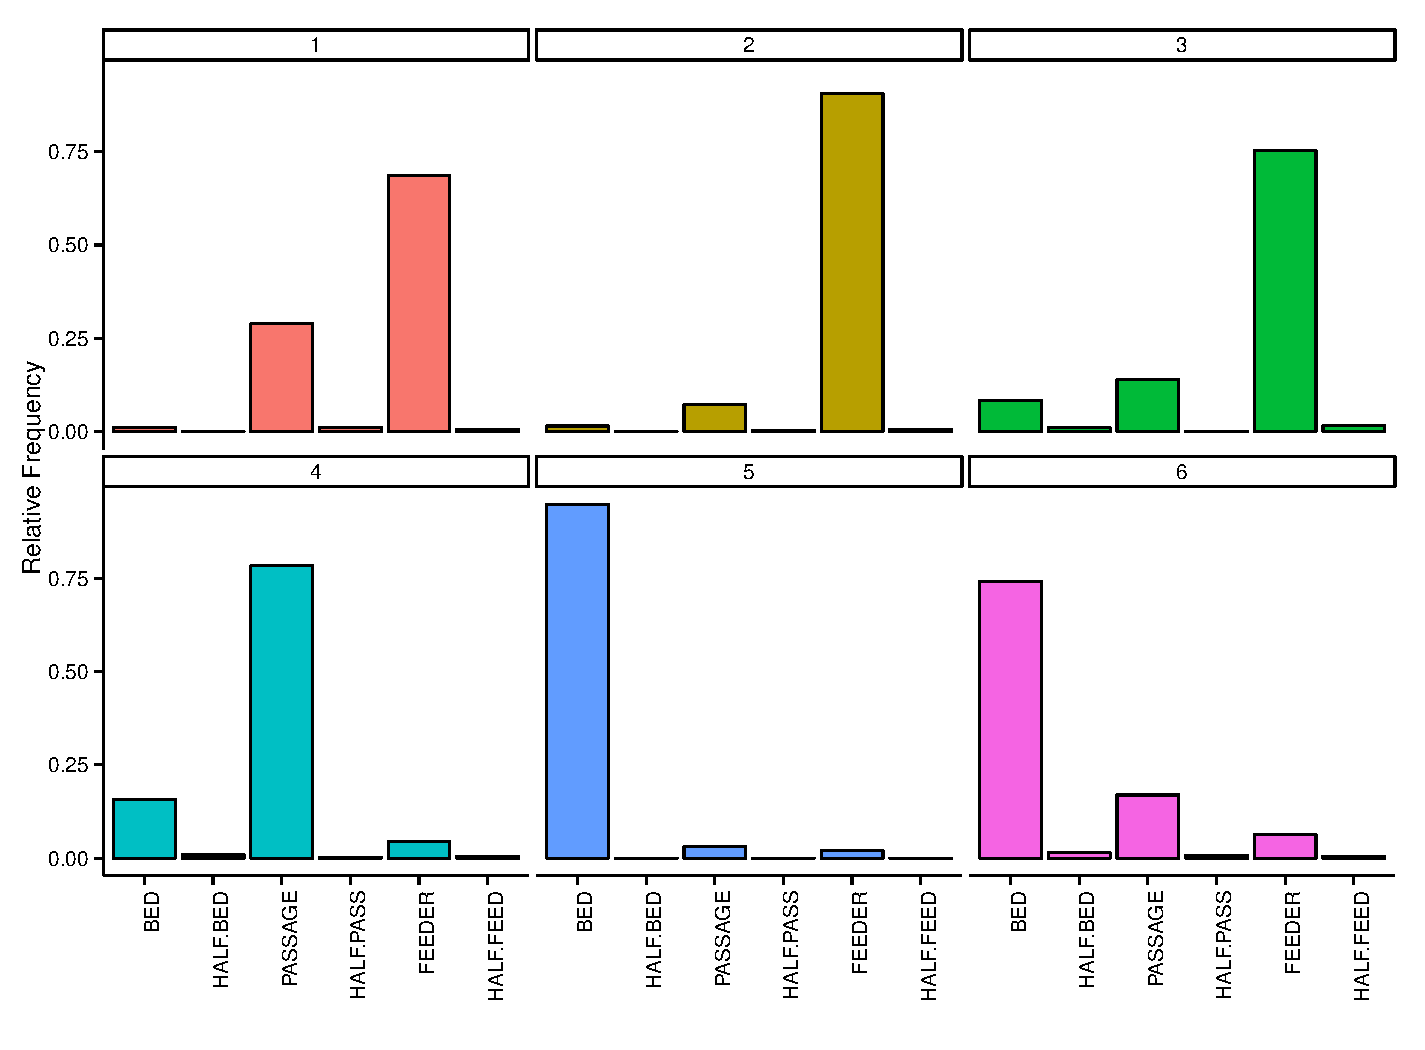
\includegraphics[width=0.95\textwidth]{figures/multinomial_mixt_all.pdf} \\
 \end{tabular}
 \caption{Components after adjusting a six mixture of multinomial distributions}\label{multinomial_mixture}
\end{center}
\end{figure}

Considering $\omega = \tau_{i I_a}$ and $\lambda = -\log^2 \left(\frac{ \tau_{iI_b} }{ \tau_{iI_a} }\right)$ we obtained the hierarchical structure partition given by


\begin{equation}
\begin{array}{r c l}
 \mathcal{P}_1&=& \{\{1,2,3,4,5,6\}\}, \\ 
 \mathcal{P}_2&=& \;\; \{\{1,2,3\},\{4,5,6\}\}, \\ 
 \mathcal{P}_3&=& \;\; \{\{1,2,3\},\{4\},\{5,6\}\}, \\ 
 \mathcal{P}_4&=& \;\; \{\{1,2\},\{3\},\{4\},\{5,6\}\}, \\ 
 \mathcal{P}_5&=& \;\; \{\{1\},\{2\},\{3\},\{4\},\{5,6\}\}, \\ 
 \mathcal{P}_6&=& \;\; \{\{1\},\{2\},\{3\},\{4\},\{5\},\{6\}\}.
\end{array}
\label{hier_ex_multinomial}
\end{equation}

Left panel of Figure~\ref{multinomial_Svalues} shows the $S$-value's obtained in each step. The $S$-values decrease with the number of clusters. In this example, with the $S$-values, it is difficult to decide the final number of clusters. To decide the final number of clusters, we used the Entropy calculated using the posterior probability vector in each step, $\sum_{i=1}^n\text{Ent}(\m\tau_{i\mathcal{P}_s})$. Using the Entropy to decide the final cluster was already suggested in \cite{baudry2010combining}. Right panel of Figure~\ref{multinomial_Svalues} shows the Entropy calculated in each step. From the plot it seems reasonable stop the merging with 3 clusters. 

\begin{figure}[t]
\begin{center}
\begin{tabular}{cc}
  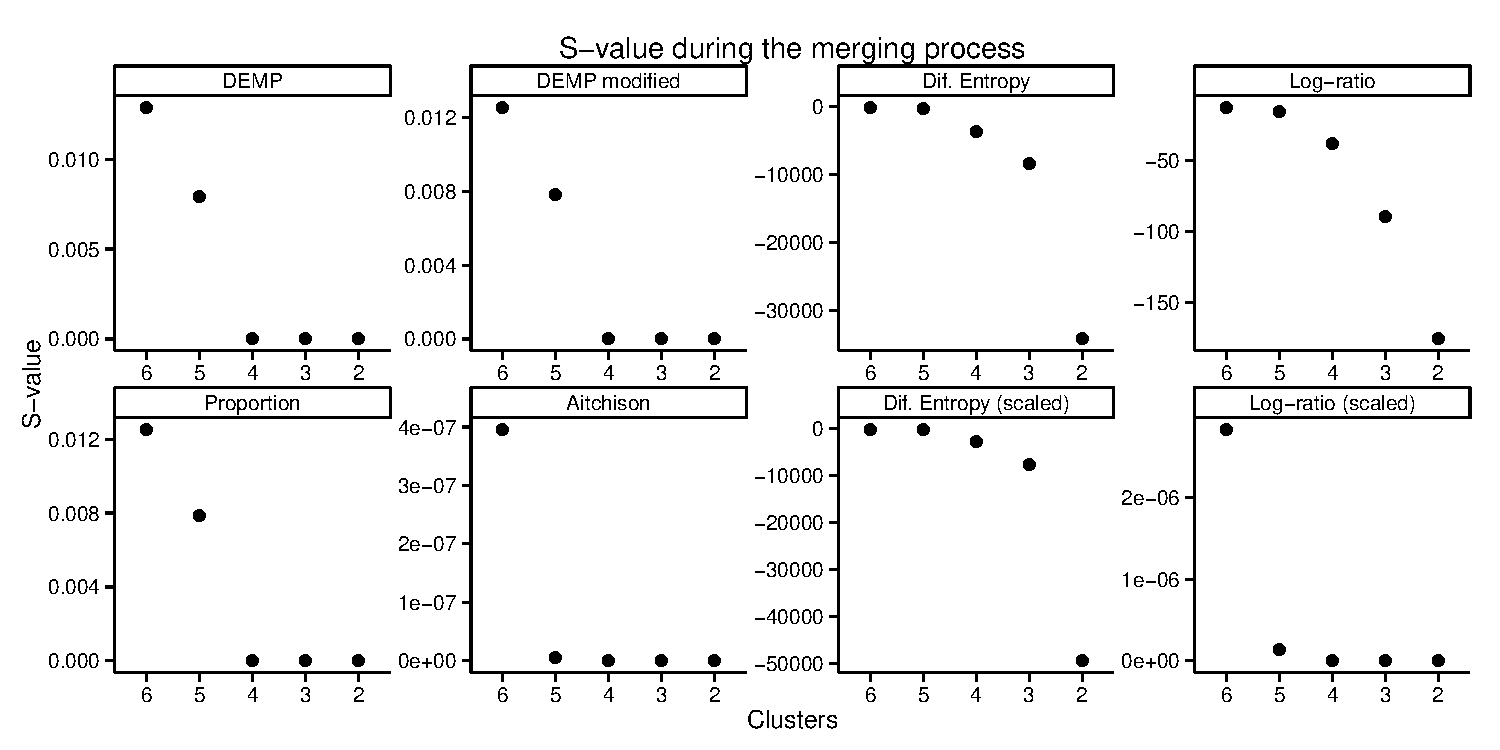
\includegraphics[width=0.85\textwidth]{figures/multinomial_Svalues_all.pdf} \\
 \end{tabular}
 \caption{S-values obtained using the Aitchison $\lambda = -\log^2 \left(\frac{ \tau_{iI_b} }{ \tau_{iI_a} }\right)$ and $\omega = \tau_{i I_a}$ in the multinomial example.}\label{multinomial_Svalues}
\end{center}
\end{figure}

Figure~\ref{multinomial_clust3} shows the final 3 clusters. The first cluster contains components 1, 2 and 4, all of them represented by sows with a high amount of time feeding. The second cluster contains components 3 and 5, this cluster is characterized by sows with high ammount of time in bed. Finally, the thirs cluster is form with a single component 6 wich have a higher amount of time in the passage.

\begin{figure}[t]
\begin{center}
\begin{tabular}{cc}
  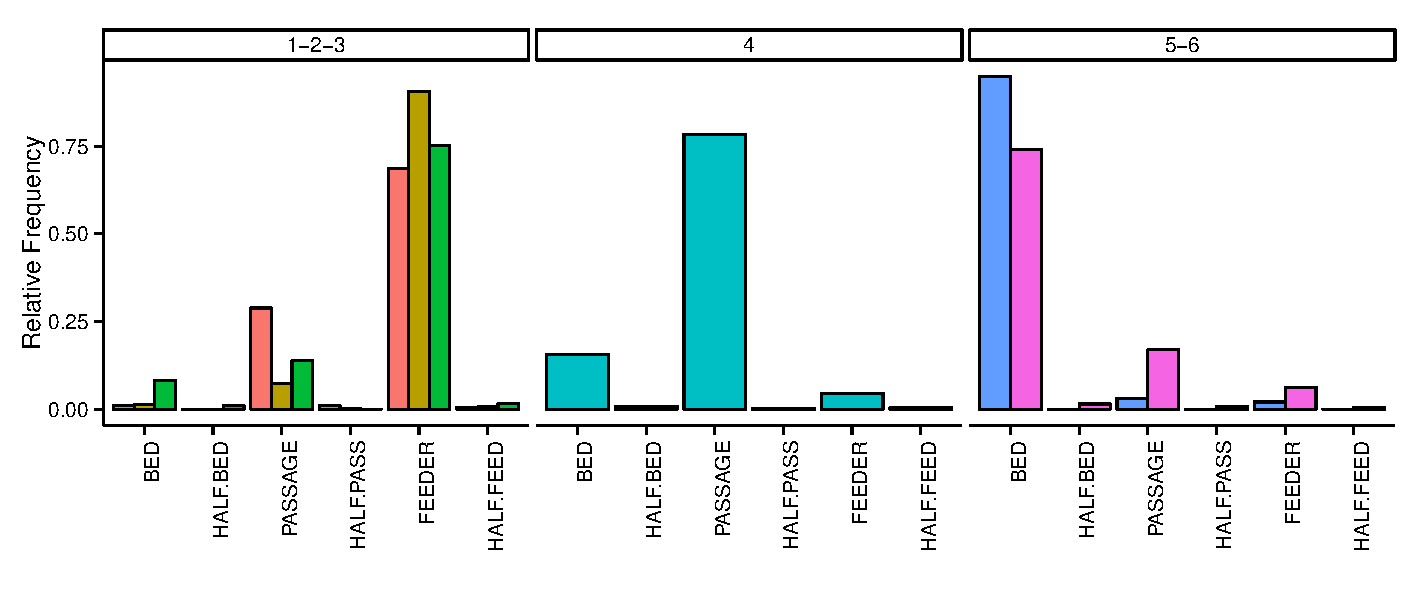
\includegraphics[width=0.95\textwidth]{figures/multinomial_clust3_all.pdf} \\
 \end{tabular}
 \caption{Components after clustering the 9 mixture components in a 3-\fmm}\label{multinomial_clust3}
\end{center}
\end{figure}

\section{Final remarks}\label{remarks}

When \fmm is used in clustering the question \textit{``is a cluster determined by a unique component?''} emerges. Different authors have proposed scenarios where it seems reasonable to argue that a cluster can be better model by more than one single component, or equivalently, modelled by a \fmm itself. In this scenarios, the approaches proposed in this article can be of interest.

In literature different approaches have been considered to merge the components of a \fmm. Some of them are specific to a particular type of mixture (methods related to gaussian mixtures) and some others are independent of the type of mixture (to cite generic approaches). The generic approach proposed in this articles only relies  on the posterior probability vectors is independent from the family of mixture and can be applied with any \fmm.

We would like to highlight the guaranteed properties obtained if the logratio approaches are considered as introduced in Section~\ref{logratio_section}: Subcompositional coherence and scale invariance. With a fixed partition $\mathcal{P}$ inside the hierarchical sequence partition, the first property allows to apply the hierarchical method to the \fmm formed with each of part of $\mathcal{P}$ separately.

Finally, the $S$-values are a reasonable measure to decide the final number of clusters when $\omega$ is constant and $\lambda = (\tau_{iI_a}+\tau_{iI_b}) \log(\tau_{iI_a} + \tau_{iI_b}) - \left\{ \tau_{iI_a} \log(\tau_{iI_a}) + \tau_{iI_b} \log(\tau_{iI_b}) \right\}$ \citep{baudry2010combining}. But the $S$-values can be missleading when other approaches are considered (Section~\ref{multinom_example}). We suggest to decide the final number of clusters using the Entropy criterion \citep{baudry2010combining}.


%%% BIBLIOGRAPHY
\newpage

\bibliographystyle{apalike}
\begin{thebibliography}{}

\bibitem[Aitchison, 1986]{aitchison1986statistical}
Aitchison, J. (1986).
\newblock {\em {The Statistical Analysis of Compositional Data}}.
\newblock Monographs on Statistics and Applied Probability. Chapman \& Hall
  Ltd., London (UK).

\bibitem[Aitchison, 2002]{aitchison2002simplicial}
Aitchison, J. (2002).
\newblock {\em {Simplicial inference}}.
\newblock {\em Algebraic Methods in Statistics anb Probability}, 287: 1--22.

\bibitem[Baudry et~al., 2010]{baudry2010combining}
Baudry, J.P., Raftery, A.~E., Celeux, G., Lo, K., and Gottardo, R. (2010).
\newblock {Combining Mixture Components for Clustering}.

\bibitem[Fraley, 2002]{fraley2002model}
Fraley, C. and Raftery, A. E. (2002).
\newblock {Model-Based Clustering, Discriminant Analysis, and Density Estimation}.
\newblock {\em Journal of the American Statistical Association}, 97(458): 611–631.

\bibitem[Hennig, 2010]{hennig2010methods}
Hennig, C. (2010).
\newblock {Methods for merging Gaussian mixture components}.
\newblock {\em Advances in Data Analysis and Classification}, 4(1):3--34.

\bibitem[Lee and Cho, 2004]{lee2004combining}
Lee, H.J. and Cho, S. (2004).
\newblock {Combining Gaussian Mixture Models}.
\newblock In Yang, Z., Yin, H., and Everson, R., editors, {\em Intelligent Data
  Engineering and Automated Learning – IDEAL 2004 SE - 98}, volume 3177 of
  {\em Lecture Notes in Computer Science}, pages 666--671. Springer Berlin
  Heidelberg.

\bibitem[Longford and Bartosova, 2014]{longford2014}
Longford, N.~T. and Bartosova, J. (2014).
\newblock {A confusion index for measuring separation and clustering}.
\newblock {\em Statistical Modelling}, 14(3):229--255.


\bibitem[McLachlan, 2014]{mclachlan2014components}
McLachlan, G. J. and Rathnayake S. (2014).
\newblock {On the number of components in a Gaussian mixture model}.
\newblock {\em Wiley Interdisciplinary Reviews: Data Mining and Knowledge Discovery},  4: 341–355.

\bibitem[Melnykov, 2013]{melnykov2013distribution}
Melnykov, V. (2013).
\newblock {On the Distribution of Posterior Probabilities in Finite Mixture
  Models with Application in Clustering}.
\newblock {\em Journal of Multivariate Analysis}, 122:175--189.

\bibitem[Palarea-Albaladejo and Martín-Fernández (2012)]{palarea2012zcompositions}
Palarea-Albaladejo J. and Martin-Fernandez J.A. (2012).
\newblock {zCompositions: Imputation of Zeros and Nondetects in Compositional Data Sets}.
\newblock {\em R package version 1.0.3}.

\bibitem[Pastore and Tonellato, 2013]{pastore2013merging}
Pastore, A. and Tonellato, S.~F. (2013).
\newblock {A Merging Algorithm for Gaussian Mixture Components}.
\newblock {\em SSRN Electronic Journal}, (04).

\bibitem[Punzo, 2014]{punzo2014flexible}
Punzo, A. (2009).
\newblock {Flexible mixture modelling with the polynomial Gaussian cluster-weighted model}.
\newblock {\em Statistical Modelling}, 14(3):257-291.

\end{thebibliography}

%%%%%%%%%%% END SPACING
%\end{spacing}

\end{document}
